%%%%%%%%%%%%%%%%%%%%%%%%%%%%%%%%%%%%%%%%%%%%%%%%%%%%%%%%%%%
%% 命令
%% \R{} R名称,暂未定义
%% \rcode 正文中的R代码,等宽字体
%% \pkg 包名称,粗体
%% \fun 函数名称,斜体
%% 大段的R代码请放在Verbatim环境中(注意是大写V不是v)

\documentclass{article}
\usepackage{ctexcap}
\usepackage{natbib}
\usepackage{array}
\usepackage{amsmath,amsthm, amsfonts, amssymb, array}
\usepackage{graphicx,booktabs,xcolor,url}
\usepackage{hyperref}
\usepackage{fancybox,fancyhdr, fancyvrb, geometry}
\usepackage{subfigure, listings}
\usepackage[toc,page]{appendix}
\newcommand{\email}[1]{\href{mailto:#1}{\normalfont\texttt{#1}}}
\newcommand{\R}{\textsf{R}}
\newcommand{\rcode}[1]{\texttt{#1}}
\newcommand{\pkg}[1]{\textbf{\textsf{#1}}}
\newcommand{\fun}[1]{\textit{#1}}
\newtheorem{exmp}{例~}
\geometry{left=3cm,right=3cm,top=2.5cm,bottom=2.5cm}
\graphicspath{{fig/}}
\RecustomVerbatimEnvironment{Verbatim}{Verbatim}{frame=leftline,numbers=left,rulecolor=\color{lightgray},framerule=4pt,numbersep=3pt}
\fvset{frame=leftline,numbers=left,rulecolor=\color{lightgray},framerule=4pt,numbersep=3pt}


\newcommand{\PreserveBackslash}[1]{\let\temp=\\#1\let\\=\temp}
\newcolumntype{C}[1]{>{\PreserveBackslash\centering}p{#1}}
\newcolumntype{R}[1]{>{\PreserveBackslash\raggedleft}p{#1}}
\newcolumntype{L}[1]{>{\PreserveBackslash\raggedright}p{#1}}
\makeatletter
\def\hlinewd#1{%
  \noalign{\ifnum0=`}\fi\hrule \@height #1 \futurelet
   \reserved@a\@xhline}
\makeatother
\setlength\arraycolsep{2pt}
\setlength{\belowcaptionskip}{3pt plus 1pt minus 2pt}


%%%%%%%%%%%%%%%%%%%%%%%%%%%%%%%%%%%%%%%%%%%%%%%%%%%%%%%%%%%%%%%%%%%
%%%%%%%%%%%%%%%%%%%%%%%%%%%%%%%%%%%%%%%%%%%%%%%%%%%%%%%%%%%%%%%%%%%
\begin{document}

\title{\heiti \R 软件在最优化中的应用}

\author{魏太云 \thanks{
	Email:weitaiyun@gmail.com;
	Homepage:\url{taiyun.cos.name} }}
\date{}
\maketitle

\begin{abstract}
最优化是一类重要问题,在科学的各个领域中都被广泛应用,免费而又强大的开源软件 \R 可以方便地
解决各类最优化问题,本文就线性规划、整数规划、目标规划、非线性规划、图与网络规划在 \R 中的求解
方法进行了初步探究。
通过研究,我们发现针对各类优化问题 (还包括较为特殊的运输问题、指派问题、旅行商问题、网络流问题等),
\R 都提供了专门的包和函数,利用它们可以简单而又完美地解决这些优化问题。同时,经过比较,我们
发现 \R 在这些优化问题的处理上要比 LINGO 软件更有优势。

\textbf{关键词:} R 软件;最优化;线性规划;整数规划;目标规划;非线性规划;图与网络规划;旅行商问题
\end{abstract}

%%%%%%%%%%%%%%%%%%%%%%%%%%%%%%%%%%%%%%%%%%%%%%%%%%%%%%%%%%%%
\section{引言}
\R \citep{R08}是一个强大、灵活、开源、免费的优秀软件,它不仅能够便捷地处理各类统计问题,而且可以毫不逊色地解决
数学规划、数据挖掘、地理信息、财政金融等诸多领域的各种问题。之所以如此,是因为
 \R 汇集了由世界上数学界、统计学界、计算机界、经济学界、物理学界、化学界、心理学界、社会学界
等各个领域的众多专家为其贡献的包,目前已经多达数千个,并且还在快速增长中。

数学规划俗称最优化,是一类非常重要的问题,在工程、地质、数学、经济、管理中都有广泛的应用。
\R 中有很多关于最优化问题的包\footnote{详情参见\url{http://cran.r-project.org/web/views
/Optimization.html},这是关于最优化包的一个总结,本文中所要用的包都可以在该网站上链接下载,
该页面的一个粗糙中译版% (由本文作者翻译) 
见\url{http://www.cos.name/bbs/read.php?tid=12135}。},
可以处理各类优化问题。本文就线性规划、整数规划、目标规划、非线性规划、图与网络规划等常见的规划问题在 \R 中的求解方法进行了初步探究,其中部分例题来自《运筹学教程》\citep{Op07}一书。
本文没有涉及太多的数学理论,而是着重讨论优化问题在软件中的解法\footnote{本文讨论都是 \R 包中已经提供了的现成解法。当然,只要我们熟悉算法和 \R 语言,我们完全可以自己编程来解决问题。}。这并不是否认算法的重要性,而是因为它们可以在大多数关于运筹学以及最优化的教程中轻松找到。此外,本文比较了 \R 和专业优化软件 LINGO 在解决各类问题的效率,其中在 LINGO 中的求解方法主要来自《运筹学--应用范例与解法》\citep{OP06}一书。

  \section{线性规划和整数规划}
 \subsection{用 \pkg{Rglpk} 包求解线性规划和整数规划}
 线性规划 (linear programming) 和整数规划\footnote{这里讨论的主要是整数线性规划,其松弛问题为线性规划。}
  (integer programming) 的主要区别是决策变量的约束不同,其中线性规划的变量为正实数,而纯整数规划的变量为正整数。
 如果决策变量中一部分为整数,另一部分可以不取整数,则该问题为混合整数规划 (mixed integer linear programming)。
 线性规划和整数规划都可以视为混合整数规划的特例,用矩阵和向量表示混合整数规划的数学模型如下:
  \begin{equation}\label{eq:lpip}
\begin{array}{l}
 \min(\text{或}\max) \ z=\mathbf{Cx}  \\
 \text{s.t.}\left\{ \begin{array}{l}
   \mathbf{Ax}\leqslant (\text{或}\geqslant, \text{或}=) \mathbf{b}\\
   \mathbf{x}\geqslant \mathbf{0}\\
   \mathbf{l} \leqslant \mathbf{X} \leqslant \mathbf{u}\\
   \mathbf{x}\ \text{中的元素取整数、 0 - 1 整数或实数}
 \end{array} \right.
 \end{array}
\end{equation}

\R 中,有很多包可以解决该问题,推荐 \pkg{Rglpk} 包\citep{Rglpk08},该包提供了到 GLPK (GNU Linear Programming Kit) 
的高级接口,不仅可以方便快速地解决大型的线性规划、整数规划、混合整数规划,并且用法非常简单。
核心函数为 \fun{Rglpk\_solve\_LP()},用法如下:

\begin{verbatim}
Rglpk_solve_LP(obj, mat, dir, rhs, types = NULL, max = FALSE,
               bounds = NULL, verbose = FALSE)
\end{verbatim}

其中,\rcode{obj} 为目标函数的系数,即模型 (\ref{eq:lpip}) 中的向量 $\mathbf{C}$,
\rcode{mat} 为约束矩阵,即模型 (\ref{eq:lpip}) 中的矩阵 $\mathbf{A}$,
\rcode{dir} 为约束矩阵 $\mathbf{A}$ 右边的符号
 (取\verb|"<"|、\verb|"<="|、\verb|"=="|、\verb|">"| 或 \verb|">="|),
\rcode{rhs} 为约束向量,即模型 (\ref{eq:lpip}) 中的向量 $\mathbf{b}$,
\rcode{types} 为变量类型,可选''B''、''I''或''C'',分别代表 0 - 1 整数变量,正整数和正实数,默认为正整数。
\rcode{max} 为逻辑参数,当其为 \rcode{TRUE} 时,求目标函数的最大值,为 \rcode{FALSE} 时 (默认),求目标函数的最小值。
\rcode{bounds} 为 \emph{x} 的额外约束,由模型 (\ref{eq:lpip}) 中向量 $\mathbf{l}$ 和 $\mathbf{u}$ 控制。
\rcode{verbose} 为是否输出中间过程的控制参数,默认为 \rcode{FALSE}。
下面通过两个例子来说明该函数的用法。
\begin{exmp}\label{ex:lpip001}
求下列简单线性规划问题。
\end{exmp}
\begin{equation*}
\begin{array}{l}
\max \ z=2 x_1 + 4 x_2 + 3 x_3\\
s.t.\left\{\begin{array}{rrrrrrr}
3x_1 &+ &4 x_2 &+ &2 x_3& \leqslant &60\\
2x_1 &+ &  x_2 &+ &  x_3& \leqslant &40\\
 x_1 &+ &3 x_2 &+ &2 x_3& \leqslant &80\\
\multicolumn{7}{l}{x_1,\  x_2, \ x_3 \geqslant 0}
\end{array}\right.
\end{array}
\end{equation*}

\noindent{{\textbf  解:}这是简单的线性规划问题,变量的类型没有特殊要求,即正实数。\R 代码及运行结果如下:}
\begin{Verbatim}
> library(Rglpk)
> obj <- c(2, 4, 3)
> mat <- matrix(c(3, 2, 1, 4, 1, 3, 2, 2, 2), nrow = 3)
> dir <- c("<=", "<=", "<=")
> rhs <- c(60, 40, 80)
> Rglpk_solve_LP(obj, mat, dir, rhs, max = TRUE)
$optimum
[1] 76.66667

$solution
[1]  0.000000  6.666667 16.666667

$status
[1] 0
\end{Verbatim}

输出结果中,\verb|$optimum| 为目标函数的最大值,\verb|$solution| 表示决策变量的最优解,
\verb|$status| 为 \rcode{0} 时,表示最优解寻找成功,非 \rcode{0} 时失败。本题中,\verb|$status| 为 \rcode{0},表示
最优解已经找到。$x_1$,$x_2$,$x_3$ 的最优解分别为 0,6.666667,16.666667,
此时目标函数取得最大值 76.66667。
\begin{exmp}\label{ex:lpip002}
求下列混合整数规划规划问题。
\end{exmp}
\begin{equation*}
\begin{array}{l}
\max \ z=3 x_1 +  x_2 + 3 x_3\\
s.t.\left\{\begin{array}{rrrrrrr}
-x_1& + & 2x_2 &+&   x_3 &\leqslant &4\\
    &   & 4x_2 &-& 3 x_3 &\leqslant &2 \\
 x_1& - & 3x_2 &+& 2 x_3 &\leqslant &3\\
\multicolumn{7}{l}{x_1,\ x_3 \ \text{为正整数}}
\end{array}\right.
\end{array}
\end{equation*}

\noindent{{\textbf  解:}这是混合整数规划问题,$x_1$,$x_3$ 为正整数,而 $x_2$ 为正实数。\R 代码及运行结果如下:}
\begin{Verbatim}
> library(Rglpk)
> obj <- c(3, 1, 3)
> mat <- matrix(c(-1, 0, 1, 2, 4, -3, 1, -3, 2), nrow = 3)
> dir <- rep("<=", 3)
> rhs <- c(4, 2, 3)
> types <- c("I", "C", "I")        ##变量类型
> Rglpk_solve_LP(obj, mat, dir, rhs, types, max = TRUE)
$optimum
[1] 26.75

$solution
[1] 5.00 2.75 3.00

$status
[1] 0
\end{Verbatim}

从输出结果可以知道,最优解已经找到 (\verb|$status| 为 \rcode{0}),$x_1$,$x_2$,$x_3$ 的最优解
为 5,2.75,3,此时目标函数取得最大值 26.75。


若变量还有定义域约束,通过设置参数 \rcode{bounds} 即可,这里不再赘述。


通过这两个例子,我们发现 \R 在解决线性规划、整数规划、混合整数规划问题时,仅仅需要将模型转换为求解函数
所需要的格式即可,并且几乎所有的约束都直接用矩阵、向量来表示,不必像 LINGO 那样需要键入 X1、X2 之类的字
符\footnote{LINGO 也可以建立向量、矩阵等数据集,但其效率不能和 \R 相提并论,因为 \R 本身就是基于数组的。}
,当问题规模较大时,这优势显得格外突出。
 \subsection{专题: \pkg{lpSolve} 包和运输问题}
 运输问题 (transportation problem) 属于线性规划问题,可以根据模型按照线性规划的方式求解,但由于其特殊性,
 用常规的线性规划来求解并不是最有效的方法。
 \pkg{lpSolve}包\citep{lpSolve08}
 提供了函数 \fun{lp.transport()} 来求解运输问题,用法如下:

 \begin{verbatim}
lp.transport(cost.mat, direction="min", row.signs, row.rhs, col.signs,
             col.rhs, presolve=0, compute.sens=0, integers = 1:(nc*nr))
\end{verbatim}
其中:


\rcode{cost.mat} 为费用矩阵,\rcode{direction} 决定求最大值还是最小值 (取 \rcode{"min"}或 \rcode{"max"})。


\rcode{row.signs}(产量约束符号,
取\verb|"<"|、\verb|"<="|、\verb|"="|、\verb|"=="|、\verb|">"| 或 \verb|">="|)和 \rcode{row.rhs}(产量约束数值) 
构成产量约束条件。


\rcode{col.signs}(销量约束符号,取\verb|"<"|、\verb|"<="|、\verb|"="|、\verb|"=="|、\verb|">"| 或 \verb|">="|)
和 \rcode{col.rhs}(销量约束数值) 构成销量约束条件。


\rcode{compute.sens} 为逻辑变量,决定是否进行灵敏度分析
 (默认为 0,即不进行灵敏度分析)。


下面通过两个例子来说明该函数的用法。
 \begin{exmp}\label{ex:trans001}
 有三个造纸厂$A_1$、$A_2$ 和 $A_3$,造纸量分别为 16 个单位、10 个单位和 22 个单位,四个客户
  $B_1$、$B_2$、$B_3$ 和 $B_4$ 的需求量分别为 8 个单位、14 个单位、12 个单位和 14 个单位。造
 纸厂到客户之间的单位运价如表 \ref{tab:trans001} 所示,确定总运费最少的调运方案。
  \begin{table}[ht]
   \caption{运费、产量及销量表}\label{tab:trans001}
   \centering
\begin{tabular}[h]{C{1.2cm}|C{1.2cm}C{1.2cm}C{1.2cm}C{1.2cm}|C{1.2cm}}
\hlinewd{1pt}
              &      $B_1$ &      $B_2$ &      $B_3$ &      $B_4$ &      产量 \\
\hline
        $A_1$ &          4 &          12 &        4 &         11 &         16 \\
%\hline
        $A_2$ &          2 &         10 &         3 &         9 &          10 \\
%\hline
        $A_3$ &          8 &          5 &         11&          6 &          22 \\
\hline
        销量 &          8 &          14 &         12&          14 &         48 \\
\hlinewd{1pt}
\end{tabular}
 \end{table}
 \end{exmp}

\noindent{{\textbf  解:}总产量等于总销量,都为 48 个单位,这是一个产销平衡的运输问题。\R 代码及运行结果如下:}
 \begin{Verbatim}
> library(lpSolve)
> costs <- matrix(c(4,2,8,12,10,5,4,3,11,11,9,6),nrow=3) #运费矩阵
> row.signs <- rep("=", 3)   #各家造纸厂的产量恰好可以售完,故都取等号
> row.rhs <- c(16,10,22)     #销量约束值
> col.signs <- rep("=", 4)   #各家客户需求量恰好可以满足,故都取等号
> col.rhs <- c(8,14,12,14)   #需求约束值
> res <- lp.transport(costs,"min",row.signs,row.rhs,col.signs,col.rhs)
> res                        #输出最小运费
Success: the objective function is 244
> res$solution               #输出运输方案
     [,1] [,2] [,3] [,4]
[1,]    4    0   12    0
[2,]    4    0    0    6
[3,]    0   14    0    8
\end{Verbatim}

 第 9 行输出结果表示问题成功解决,最少运费为 244,第 11 -- 14 行为输出的运输矩阵,运送方案为:
  $A_1\rightarrow B_1$ : 4 个单位,$A_1\rightarrow B_3$ : 12 个单位,$A_2\rightarrow B_1$ : 4 个单位,
  $A_2\rightarrow B_4$ : 6 个单位,$A_3\rightarrow B_2$ : 14 个单位,$A_3\rightarrow B_4$ : 8 个单位。


 下面再看一个产销不平衡的运输问题。
%%%%-----------------------------------------------------------------------------
 \begin{exmp}\label{ex:trans002}
 有三个造纸厂 $A_1$、$A_2$ 和 $A_3$ ,造纸量分别为 8 个单位、5 个单位和 9 个单位,四个客户
  $B_1$、$B_2$、$B_3$ 和 $B_4$ 的需求量分别为 4 个单位、3 个单位、5 个单位和 6 个单位。造纸
 厂到客户之间的单位运价如表 \ref{tab:trans002} 所示,确定总运费最少的调运方案。
  \begin{table}[ht]
   \caption{运费、产量及销量表}\label{tab:trans002}
   \centering
\begin{tabular}[h]{C{1.2cm}|C{1.2cm}C{1.2cm}C{1.2cm}C{1.2cm}|C{1.2cm}}
\hlinewd{1pt}
              &      $B_1$ &      $B_2$ &      $B_3$ &      $B_4$ &      产量 \\
\hline
        $A_1$ &          3 &          12 &        3 &         4 &         8 \\
%\hline
        $A_2$ &          11 &         2 &         5 &         9 &         5 \\
%\hline
        $A_3$ &          6 &          7 &         1&          5 &         9 \\
\hline
        销量 &          4 &          3 &         5 &          6 &          \\
\hlinewd{1pt}
\end{tabular}
%\end{center}
\end{table}
\end{exmp}
\noindent{{\textbf  解:} 总产量为 $8+5+9=22$ 个单位,而总销量为 $4+3+5+6=18$ 个单位,总产量大于总销量,故这是
 一个产销不平衡的运输问题。这和上一题的主要区别是产量约束符号不再都为等号,而是根据实际情况取相应的符号。
 \R 代码及运行结果如下:}
 \begin{Verbatim}
> costs <- matrix (c(3,11,6,12,2,7,3,5,1,4,9,5),nrow=3); ##运费矩阵
> row.signs <- rep ("<=", 3)   #总产量大于总销量,故各家销量小于等于产量
> row.rhs <- c(8,5,9)          #销量约束值
> col.signs <- rep ("=", 4)    #各家客户需求量都可以满足,故都取等号
> col.rhs <- c(4,3,5,6)        #需求约束值
> res <- lp.transport(costs,"min",row.signs,row.rhs,col.signs,col.rhs)
> res                          #输出最小运费
Success: the objective function is 49
> res$solution                 #输出运输方案
     [,1] [,2] [,3] [,4]
[1,]    4    0    0    4
[2,]    0    3    0    0
[3,]    0    0    5    2
 \end{Verbatim}

 从运行结果可以看出,问题成功解决,最少运费为 49,运输方案为:
  $A_1 \rightarrow 
 B_1$ : 4 个单位,$A_1\rightarrow
 B_4$ : 4 个单位,$A_2\rightarrow
 B_2$ : 3 个单位,$A_3\rightarrow
 B_3$ : 5 个单位,$A_3\rightarrow
 B_4$ : 2 个单位。


对于其它产销不平衡问题,根据具体情况 (如果有必要的的话,则进行适当的变换),
调用函数 \fun{lp.transport()} 来求解。


LINGO 在求解运输问题时,要通过各种命令建立数据集、模型、目标函数、约束函数等,比较
繁琐%\footnote{详见由 Wayne L. Winston 所著的《运筹学--应用范例与解法》第 413 页,第四版,清华大学出版。}
,相比之下,\R 的代码显得简洁而又直观。
\subsection{专题: \pkg{lpSolve} 包和指派问题}
 指派问题 (assignment problem) 属于 0 - 1 整数规划,是一种特殊的整数规划问题。指派问题的标准形式 (以人和事为例) 是:
 有 n 个人和 n 个事,已知第 i 个人做第 j 件事的费用为 $c_{ij}\ (i,j=1,2,\cdots,n)$,要求确定人和事之间
 的一一对应的指派方案,使完成 n 件事的总费用最少。


 \R 中, \pkg{lpSolve} 包
 提供了函数 \fun{lp.assign()} 来求解标准指派问题,
 其用法如下:

\begin{verbatim}
lp.assign (cost.mat,direction = "min", presolve = 0, compute.sens = 0)
\end{verbatim}

 其中,\rcode{cost.mat} 为指派问题的系数矩阵,其元素的意义根据实际情况而定,可以是费用、时间、
 成本等。\rcode{direction} 为逻辑变量,来决定求总费用的最大值还是最小值,默认求总
 费用的最小值。\rcode{compute.sens} 决定是否进行灵敏度分析。
 \begin{exmp}\label{ex:ap}
 某商业公司计划开办 5 家新商店。为了尽早建成营业,商业公司决定由 5 家建筑公司分别承建。已知建筑公司
  $A_i(i=1,2,\cdots,5)$ 对新商店 $B_j(j=1,2,\cdots,5)$ 的建造费用的报价 (万元) 为 $c_{ij}(i,j=1,2,\cdots,5)$,
 如表 \ref{tab:assign}。该公司应对 5 家建筑公司怎样分配建筑任务,才能使总的建筑费用最少?
 \begin{table}[h]
  \caption{建筑费用报价表}\label{tab:assign}
  \centering
 % \begin{center}
\begin{tabular}{C{1.2cm}|C{1.2cm}C{1.2cm}C{1.2cm}C{1.2cm}C{1.2cm}}
\hlinewd{1pt}
              &      $B_1$ &      $B_2$ &      $B_3$ &      $B_4$ &      $B_5$ \\
\hline
        $A_1$ &          4 &          8 &          7 &         15 &         12 \\
%\hline
        $A_2$ &          7 &          9 &         17 &         14 &         10 \\
%\hline
        $A_3$ &          6 &          9 &         12 &          8 &          7 \\
%\hline
        $A_4$ &          6 &          7 &         14 &          6 &         10 \\
%\hline
        $A_5$ &          6 &          9 &         12 &         10 &          6 \\
\hlinewd{1pt}
\end{tabular}
%\end{center}
 \end{table}
  \end{exmp}

\noindent{{\textbf  解:}这是一个标准的指派问题。\R 代码及运行结果如下:}
\begin{Verbatim}
> library(lpSolve)
> x=matrix(c(4,7,6,6,6,8,9,9,7,9,7,17,12,14,12,
+            15,14,8,6,10,12,10,7,10,6),ncol=5)  ##指派问题的系数矩阵
> lp.assign(x)
 Success: the objective function is 34
> lp.assign(x)$solution
     [,1] [,2] [,3] [,4] [,5]
[1,]    0    0    1    0    0
[2,]    0    1    0    0    0
[3,]    1    0    0    0    0
[4,]    0    0    0    1    0
[5,]    0    0    0    0    1
\end{Verbatim}

从运行结果可以看出,最优解已经成功找到。由 \verb|lp.assign(x)$solution| 得知,
最优指派方案是:$A_1$ 承建 $B_3$,$A_2$ 承建 $B_2$,$A_3$ 承建 $B_1$,$A_4$ 承建 $B_4$,
$A_5$ 承建 $B_5$。这样安排能使总费用最少,为 $7+9+6+6+6=34$ 万元。


在实际应用中,常会遇到各种非标准形式的指派问题,有时不能直接调用函数,处理方法是将它们化为标准
形式\citep{Op07},然后再通过标准方法求解。


同运输问题一样,LINGO 在解决指派问题时,也必须通过各种命令建立数据集、模型、目标函数、约束函数等,比较
繁琐%\footnote{详见由 Wayne L. Winston 所著的《运筹学--应用范例与解法》第 442 页,第四版,清华大学出版。}
,相比之下,\R 两三句代码就可以快速解决问题,较之 LINGO 软件,的确方便快捷了许多。
%%%线性规划整数规划
  \section{目标规划}
 \subsection{目标规划问题及其数学模型}
 目标规划\footnote{目标规划可分为线性和非线性两种,这里讨论的是比较简单的线性目标规划 
(linear goal programming)。} (goal programming) 是运筹学中的一个重要分支,它是为解决多目标决策问题而发展起来
 的一种数学方法。目标规划可以按照确定的若干目标值及其实现的优先次序,在给定约束条件下寻找
 偏离目标值最小的解的数学方法。它在处理实际决策问题时,承认各项决策要求 (即使是冲突的) 
 的存在有合理性;在做最终决策时,不强调其绝对意义上的最优性。由于目标规划在一定程度上弥补了线性规划
 的局限性,因此,目标规划被认为是一种较之线性规划更接近于实际决策工程的工具。


 目标规划数学模型的一般形式为:
 \begin{equation}\label{eq:gp}
\begin{array}{ll}
 \min P_l (\sum\limits_{k = 1}^K ({W_{lk}^- d_k^- + W_{lk}^ +  d_k^+  } ))&l=1,2,\ldots,L \\
 \multicolumn{2}{l}{\text{s.t.}
 \left\{ \begin{array}{ll}
\sum\limits_{j = 1}^n {c_{kj}x_j+ d_k^- -d_k^+ }=g_k            &k = 1,2,\ldots,K \\
\sum\limits_{j = 1}^n {a_{ij}x_j \leqslant(\text{或}=,\text{或}\geqslant) b_i}     &i = 1,2,\ldots,m \\
 x_j  \geqslant 0&j = 1,2,\ldots,n \\
 d_k^ - ,\ d_k^+ \geqslant 0                                   &k = 1,2,\ldots,K \\
 \end{array} \right.}
 \end{array}
\end{equation}

模型 (\ref{eq:gp}) 的约束条件中,第一行有偏差变量,为目标约束,第二行没有偏差变量,同线性规划里的约束条件一样,
为绝对约束。可以证明,
在模型 (\ref{eq:gp}) 有解的情况下,可以将其化为只含有目标约束的目标规划问题,方法是给所有的绝对约束赋予足够
高级别的优先因子,从这个角度来看,线性规划为目标规划的特殊情况,而目标规划则为线性规划的自然推广。
根据以上分析,可将模型 (\ref{eq:gp}) 简化并用矩阵和向量记为:
\begin{equation}\label{eq:gp2}
\begin{array}{ll}
 \min \mathbf{P}(\mathbf{W}^- \mathbf{d}^- +\mathbf{W}^+ \mathbf{d}^+)\\
 \text{s.t.}{\left\{ \begin{array}{l}
 \mathbf{Ax}+ \mathbf{d}^- -\mathbf{d}^+=\mathbf{g}       \\
 \mathbf{d}^- ,\ \mathbf{d}^+ \geqslant\mathbf{0}     \\
 \mathbf{x} \geqslant \mathbf{0}                  \\
 \end{array} \right.}
 \end{array}
\end{equation}

模型 (\ref{eq:gp2}) 中,所有的约束都为目标约束,每一个目标约束都对应一对偏差变量。

\subsection{用 \pkg{goalprog} 包求解目标规划}

\R 中, \pkg{goalprog} 包\citep{goalprog08}可以求解形式为模型 (\ref{eq:gp2}) 的目标规划问题,
核心函数为 \fun{llgp()},用法如下:
\begin{verbatim}
llgp(coefficients, targets, achievements, maxiter = 1000, verbose = FALSE)
\end{verbatim}

参数中,\rcode{coefficients} 为约束变量 (不包括偏差变量) 的系数矩阵,即模型 (\ref{eq:gp2}) 中的矩阵 $\mathbf{A}$。
\rcode{targets} 为系数矩阵对应的约束向量,即模型 (\ref{eq:gp2}) 中的向量 $\mathbf{g}$。
\rcode{achievements} 为关于目标函数 (默认求最小值) 的数据框,是由 4 个向量构成:objective、priority、
p 和 n。其中数据框的每一行对应一个软约束条件,objective 和 priority 为正整数,分别表示针对第几对偏差变量
 (第 n 对偏差变量必须出现在第 n 个目标约束中) %%%%%%%%%变量 (次序和一致) 该目标约束对应的
和该偏差变量的优先级别 ,p 和 n 分别表示 $d^+$(正偏差变量)、$d^-$(负偏差变量) 的权
系数\footnote{p 和 n 分别为 positive (正的) 和 negative (负的) 的首字母,这与它们代表的偏差变量的正负是一致的。}。
\rcode{maxiter} 为最大迭代次数,取正整数,默认为 1000。
\rcode{verbose} 为逻辑变量 (取 \rcode{TRUE} 或 \rcode{FALSE} ),决定是否输出中间过程,默认不输出。
\begin{exmp}
(来自 \citep{Op07} 例题 4.2) 某工厂生产两种产品,受到原材料供应和设备工时的限制,在单位利润等有关数据已知的条件下,要求制定一个获利最大的
生产计划,具体数据见表 \ref{tab:gp001}。


 \begin{table}[ht]
   \caption{生产约束、利润表}\label{tab:gp001}
   \centering
\begin{tabular}[h]{L{3cm}|C{2cm}|C{2cm}|C{2cm}}
\hlinewd{1pt}
        产品\centering &      A &          B &     限量  \\
\hline
        原材料 (kg/件) &      5 &         10 &       60\\
%\hline
        设备工时 (h/件)&      4 &           4&       40 \\
%\hline
        利润 (元/件)   &      6 &          8 &        \\
\hlinewd{1pt}
\end{tabular}
 \end{table}
 \end{exmp}

在决策时,按重要程度的先后顺序,要考虑如下意见:
\begin{enumerate}
\item 原材料严重短缺,生产中应避免浪费,不得突破使用限额;
\item 由于产品 B 销售疲软,故希望产品 B 的产量不超过产品 A 的一半;
\item 最好能节约 4 h 的设备工时;
\item 计划利润不少于 48 元。
\end{enumerate}

以上四条意见中,显然第一条为绝对约束,第二至四条为目标约束。
请根据这些要求决定两种产品生产量。


\noindent{{\textbf  解:}这是典型的多目标规划问题,建立目标规划模型如下:}

\begin{equation*}
\begin{array}{l}
 \min \ \{P_1d_1^-,\ P_2d_2^+,\  P_3d_3^-\}\\
 \text{s.t.}\left\{ \begin{array}{rrrrrrrrr}
 5x_1&+ & 10x_2 &  &        & &        &\leqslant& 60\\
  x_1&- &   x_2 &+ &d_1^{-} &-& d_1^{+}&        =&  4\\
 4x_1&+ &  4x_2 &+ &d_2^{-} &-& d_2^{+}&        =& 56\\
 6x_1&+ &  8x_2 &+ &d_3^{-} &-& d_3^{+}&        =& 12\\
 \multicolumn{9}{l}{x_1, \ x_2,\  d_{1-3}^-, \ d_{1-3}^{+}\ \geqslant0}
 \end{array} \right.
 \end{array}
\end{equation*}

该模型中含绝对约束条件,将绝对约束条件转化为一级目标约束条件,得到模型如下:
\begin{equation*}
\begin{array}{l}
 \min \ \{P_1d_1^+,\ P_2d_1^-,\ P_3d_2^+,\  P_4d_3^-\}\\
 \text{s.t.}\left\{ \begin{array}{rrrrrrrrr}
 5x_1&+ & 10x_2 & +&d_1^{-} &-& d_1^{+}&\leqslant& 60\\
  x_1&- &   x_2 &+ &d_2^{-} &-& d_2^{+}&        =&  4\\
 4x_1&+ &  4x_2 &+ &d_3^{-} &-& d_3^{+}&        =& 56\\
 6x_1&+ &  8x_2 &+ &d_4^{-} &-& d_4^{+}&        =& 12\\
 \multicolumn{9}{l}{x_1, \ x_2,\  d_{1-4}^-, \ d_{1-4}^{+}\ \geqslant0}
 \end{array} \right.
 \end{array}
\end{equation*}

该模型符合模型 (\ref{eq:gp2}) 的形式,可以直接调用 \fun{llgp()} 函数来求解该问题,
注意:\R 中根据 \rcode{achievements} 数据框
中的 priority 来判断绝对优先级别,不用再设置 $P_1$,$P_2$,$P_3$。\R 代码和部分输出结果如下:
\begin{Verbatim}
> library(goalprog)
> coefficients=matrix(c(5,1,4,6,10,-2,4,8),4)
> targets=c(60,0,36,48)
> achievements=data.frame(objective=1:4,priority=c(1,2,3,4),
+                         p=c(1,0,1,0),n=c(0,1,0,1))
> soln=llgp(coefficients, targets, achievements)
> soln$converged
[1] TRUE
> soln$out

Decision variables
                X
X1   4.800000e+00
X2   2.400000e+00
\end{Verbatim}

观察输出结果,可以知道该问题已经得到最优解 (\verb|soln$converged| 为 \rcode{TRUE} 时,表示最优解已经找到),
此时 $x_1$,$x_2$ 分别取 4.8,2.4,即应生产 A 产品 4.8 个单位,B 产品 2.4 个单位。需要说明的是,由于约束较少,
本题有四个满意解,这里仅仅得到一个。此外,
程序结果输出较多,上面的 \verb|soln$out| 仅选取了一部分。
下面再看一个稍微复杂的例子。
\begin{exmp}
求下列目标规划问题:
 \begin{equation*}
\begin{array}{l}
 \min \ \{P_1(2d_1^+ + 3d_2^+),\ P_2d_3^-,\  P_3d_4^+\}\\
 \text{s.t.}\left\{ \begin{array}{rrrrrrrrr}
 x_1&+ & x_2 &+ &d_1^{-} &-& d_1^{+}&=& 10\\
 x_1&  &     &+ &d_2^{-} &-& d_2^{+}&=& 4\\
 5x_1&+& 3x_2&+ &d_3^{-} &-& d_3^{+}&=& 56\\
 x_1&+ & x_2 &+ &d_4^{-} &-& d_4^{+}&=&12\\
 \multicolumn{9}{l}{x_1, \ x_2,\  d_{1-4}^-, \ d_{1-4}^{+}\ \geqslant 0}
 \end{array} \right.
 \end{array}
\end{equation*}
\end{exmp}

\noindent{{\textbf  解:}这是一个多目标规划问题,可以直接调用 \fun{llgp()} 函数求解。
\R 代码及运行结果如下 (为了便于展示,输出了一些参数的信息):}
\VerbatimInput{./code/gp3.r}

分析输出结果,可以知道该问题已经得到最优解,
此时 $x_1$,$x_2$ 分别为 4,6。


通过这两个例子,我们发现该函数在解决目标规划问题上非常简捷,只需要套用格式,将问题转化为
函数需要的格式即可。而 LINGO 在求解目标规划时则比较笨拙,它需要将多目标转化为单目标,当
目标函数比较复杂时,这一过程将会非常繁琐而又困难。
%%%目标规划
  \section{非线性规划}
 \subsection{非线性规划问题及其数学模型}
非线性规划 (non-linear programming) 问题不要求目标函数、约束条件都为线性形式,较之线性规划问题以及由其发展出来的整数规划、目标规划,
非线性规划的应用更加广泛,一般的线性规划仅仅是非线性规划的特例而已。由于约束条件的放宽,非线性规划问题可以
更接近于现实生活中的种种问题,同时,求解难度也提高了很多。用矩阵和向量来表示非线性函数的数学模型如下:
 \begin{equation}\label{eq:nlp}
\begin{array}{l}
 \min \ z=f({\mathbf{x}})  \\
 \text{s.t.}\left\{ \begin{array}{ccccc}
   \mathbf{x_l}& \leqslant&    \mathbf{x}  & \leqslant  & \mathbf{x_u} \\
   \mathbf{b_l}& \leqslant&   \mathbf{Ax}  & \leqslant  & \mathbf{b_u} \\
   \mathbf{c_l}& \leqslant&  \mathbf{c(x)} & \leqslant  & \mathbf{c_u}\\
 \end{array} \right.
 \end{array}
\end{equation}

模型 (\ref{eq:nlp}) 中,$z=f(\mathbf{x})$ 为目标函数,三个约束条件中,第一个为定义域约束,第二个为线性约束 ($\mathbf{A}$ 为系数矩阵),
第三个为非线性约束\footnote{注意:$\mathbf{c(x)}$ 为一组非线性约束函数,而不局限于一个。}。当目标函数和
约束函数光滑时,称之为光滑的非线性规划,其求解的难度要小于非光滑的非线性规划。
\subsection{用 \pkg{Rdonlp2} 包求解光滑的非线性规划}
对于无约束或者约束条件相对简单的非线性优化问题,\pkg{stats} 包中的 \fun{optim()}、\fun{optimize()}、 
 \fun{constrOptim()}、\fun{nlm()}、\fun{nlminb()} 等函数可以完美地解决,并且它们的使用方法相当简单。
 鉴于该包为默认安装包,大多数人比较熟悉,下面着重探讨专门解决非线性优化的 \pkg{Rdonlp2} 包\citep{Rdonlp207}
 的用法。


\R 中,\pkg{Rdonlp2} 包是一个非常强大的包,可以方便快速地解决光滑的非线性规划问题。该包在学习、研究中可以自由
使用,其它用途则需要授权。核心函数为 \fun{donlp2()},可以求连续非线性函数的最值 (默认求最小值) ,用法如下:

\begin{verbatim}
 donlp2(par, fn,
        par.upper=rep(+Inf, length(par)),
        par.lower=rep(-Inf, length(par)),

        A = NULL,
        lin.upper=rep(+Inf, length(par)),
        lin.lower=rep(-Inf, length(par)),

        nlin = list(),
        nlin.upper=rep(+Inf, length(nlin)),
        nlin.lower=rep(-Inf, length(nlin)),

        control=donlp2.control(),
        control.fun=function(lst){return(TRUE)},
        env=.GlobalEnv,
        name="Rdonlp2")
\end{verbatim}

该函数的参数较多,下面分类对它们进行详细解释:
\begin{enumerate}
\item 初始值、目标函数及自变量定义域:
\begin{description}
\item [par] 向量,迭代初始值。
\item [fn] 连续型函数,函数自变量限制为 1 个 (自变量一般为向量,这样可以包含多个参数),函数的返回值
                 为优化目标。
\item [par.upper 和 par.lower] 向量,分别为自变量的上下界限,即模型 (\ref{eq:nlp}) 中的
                 $\mathbf{x_u}$ 和 $\mathbf{x_l}$,它们的长度应该和向量 \rcode{par} 
                相等。如果变量无界,必须用正无穷 (+Inf) 和负无穷大 (-Inf) 来表示。可以看出,自变量默认
                无界,可以取全体实数。
\end{description}

\item 线性约束:
\begin{description}
\item [A]线性约束矩阵,即模型 (\ref{eq:nlp}) 中的矩阵 $\mathbf{A}$,其列的长度必须和向量 \rcode{par} 相等 (即总变量个数),
            其行的长度必须和线性约束的个数相等。
\item [lin.upper 和 lin.lower]向量,分别为线性约束条件的上下界限,即模型 (\ref{eq:nlp}) 中的
                 $\mathbf{b_u}$ 和 $\mathbf{b_l}$,它们的长度应该和线性约束的个数相等。
                如果某个线性约束无界,必须用正无
                穷 (+Inf) 
                或负无穷大 (-Inf) 来表示。如果某一个线性约束取固定值,那么只要设置它在 \rcode{lin.upper} 和
                 \rcode{lin.lower} 两个向量中对应
                位置都为该固定值即可 (如 $ax_1+bx_2=k$,可化为 $k\leqslant ax_1+bx_2 \leqslant k$,即上下界都为 k),
                这方法同样适合于下面要说的非线性约束条件的控制。
\end{description}
\item 非线性约束:
\begin{description}
\item [lin]列表,其中的元素为表示非线性约束条件的函数。
\item [nlin.upper 和 nlin.lower]向量,分别为非线性约束条件的上下界限,即模型 (\ref{eq:nlp}) 中的
                 $\mathbf{c_u}$ 和 $\mathbf{c_l}$,它们的长度应该和非线性约束的个数相等。
                如果某个非线性约束无界,必须用正无穷 (+Inf) 
                或负无穷大 (-Inf) 来表示。
\end{description}

\item 控制参数:
\begin{description}
\item[control]     控制参数,为 donlp2.control(),可以修改一些关于算法的参数和输出参数,可以根据实际要求修改。
\item[control.fun] 控制函数。
\item[env]  运行环境,一般不需要更改。
\item[name] 字符变量,如果不是默认值,则会在程序运行时在工作目录生成两个以 \rcode{name} 为主文件名,
            后缀分别为 pro、mes 的文件,其中 name.pro 文件为优化问题运行结果,name.mes 文件为警告及其它信息。
\end{description}
\end{enumerate}
 \begin{exmp}
求下列有约束的非线性规划问题。
\begin{equation*}
\begin{array}{l}
 \min \ z=x^2\sin y  + y^2\cos x  \\
 s.t.\left\{ \begin{array}{l}
  - 100 < x < 100 \\
  - 100 < y < 100 \\
  1\leqslant 3x - y   \leqslant 3\\
  x  + y   \geqslant 2\\
  \sin x\cos y \leqslant 0.6\\
  xy = 2
 \end{array} \right.
 \end{array}
\end{equation*}
 \end{exmp}
\noindent{{\textbf  解:}这是一个非线性规划问题。R 代码如下:}
\begin{Verbatim}
library(Rdonlp2)                          #载入包
p = c(10,10)                              #迭代初始值
par.l= c(-100,-100); par.u = c(100,100)   #自变量定义域约束
fn = function(x){
  x[1]^2*sin(x[2])+x[2]^2*cos(x[1])
}                                         #目标函数
A = matrix(c(1,1,3,-1),2,byrow=TRUE)
lin.l = c(2,1);lin.u = c(+Inf,3)          #7-8行构成线性约束
nlcon1 = function(x){
  x[1]*x[2]
}
nlcon2 = function(x){
  sin(x[1])*cos(x[2])
}
nlin.l = c(2,-Inf)
nlin.u = c(2,0.6)                          #9-16行构成非线性约束
ret = donlp2(p, fn, par.u=par.u, par.l=par.l,A,lin.l=lin.l,lin.u=lin.u,
             nlin=list(nlcon1,nlcon2), nlin.u=nlin.u, nlin.l=nlin.l)
\end{Verbatim}

运行程序,从输出结果\footnote{输出结果很多,有关于运行时间的,有关于中间过程的,也有关于算法参数的,在此
仅列出最感兴趣的输出。}中可以找到下面结果:
\begin{Verbatim}
 KT-conditions satisfied, no further correction computed
 optimal value of f =   2.28705347564892e+00
 optimal solution x =
  1.40307592849219e+00  1.42543960692795e+00
\end{Verbatim}

其中第 1 行表示求解成功,第 2 行表示此时目标函数最小值为 2.287(保留三位小数,后面也是如此),3 - 4 行
表示 x,y 分别为 1.403,1.425。


下面利用该包求解 Rastrigin 函数的最小值,由于该函数族极值点很多,而最值点仅有一个,
因而被广泛运用于测试各类优化算法,先选择一个二元的 Rastrigin 函数:
\[
 \min \ f(X) = \sum\limits_{i = 1}^2 {(x_i^2  - 10\cos (2\pi x_i ) + 10)}
\]

首先画出该函数在 x,y 区间都为 $[-5,5]$ 时的三维曲面图和颜色图,程序如下:
\begin{Verbatim}
a = 5
x = seq(-a, a, 0.01)
y = seq(-a, a, 0.01)
f = function(x, y){
    x^2 - 10*cos(2*pi*x) + y^2 - 10*cos(2*pi*y) + 20
}
z = outer(x, y, f)
image(x,y,z, col=heat.colors(24))      #画颜色图
library(rgl)                           #该包可以画出漂亮的三维曲面图
zorder = rank(z)
persp3d(x, y, z, col = rainbow(as.integer(max(zorder)))[zorder])
\end{Verbatim}
\begin{figure}
\begin{minipage}[t]{0.50\linewidth}
\centering
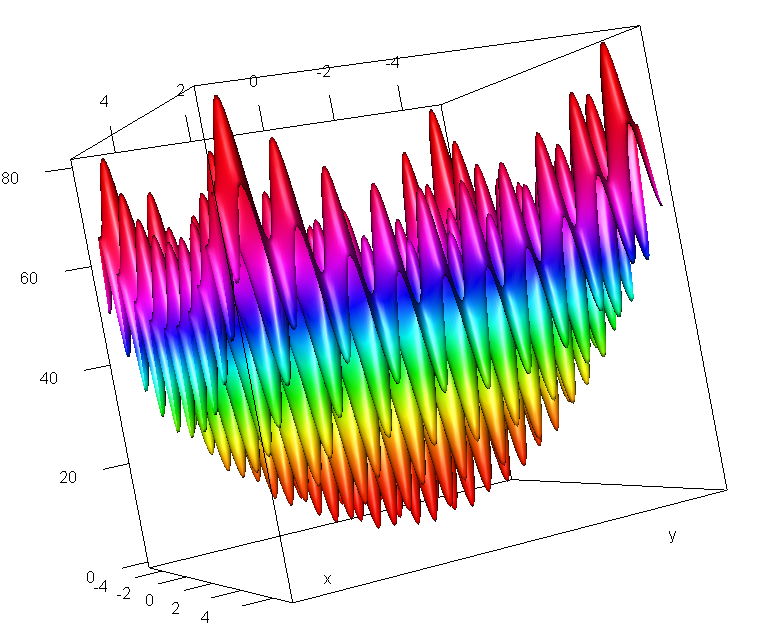
\includegraphics[width=\textwidth]{./pic/dim3.png}
\caption{三维曲面图 \label{fig:sanwei}}
\end{minipage}
\hfill
\begin{minipage}[t]{0.50\linewidth}
\centering
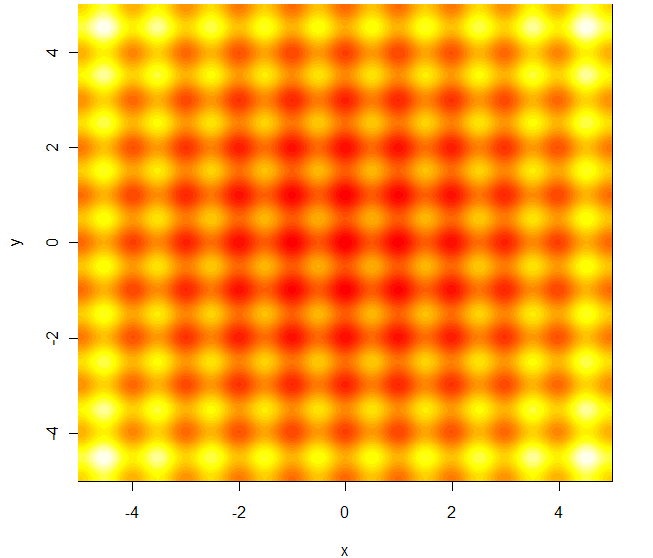
\includegraphics[width=\textwidth]{./pic/a.png}
\caption{颜色图\label{fig:color}}
\end{minipage}
\end{figure}

图 \ref{fig:sanwei} 为 Rastrigin 函数的三维曲面图,从图中可以看出,曲面图在该区域内
 (这里才仅仅取了很小的区域!) 有很多“尖刺”,这些“尖刺”就是极值点。
图 \ref{fig:color} 为 Rastrigin 函数的颜色图,函数值越小,颜色越深。红色点 (即深色点) 
即为局部极小点,可以看出仅仅在该区域内,函数已经有 121 个极小点了,这就使得 Rastrigin 函数最小点的求解变
得非常困难。现在用 \pkg{Rdonlp2} 包来求该函数的最小点。\\
{\textbf  解:}R 代码和部分运行结果如下:
\begin{Verbatim}
> library(Rdonlp2)
> fn=function(x){
>   f=sum(x^2-10*cos(2*pi*x)+10)  ##Rastrigin函数,参数x为向量,长度不定
> }
> par=c(-500,+500)                ##随便定义一个偏离最优解较远的初时迭代向量
> ret=donlp2(par,fn)
 optimal value of f =   0.00000000000000e+00

 optimal solution  x =
  3.31453975377372e-10 -3.31453975377372e-10
\end{Verbatim}

运行程序,可以发现最优解成功找到,目标函数最小值为 0(此时$x=0$,$y=0$),所耗时间极短。可以看出,\pkg{Rdonlp2} 
包处理该优化问题游刃有余,现在增加难度,求解有 1000 个变量的 Rastrigin 函数的最小值:
\[
 \min \ f(X) = \sum\limits_{i = 1}^{1000} {(x_i^2  - 10\cos (2\pi x_i ) + 10)}
\]

在 1000 维空间中,该函数的极小点奇多无比,求解非常困难。程序代码如下:
\begin{Verbatim}
library(Rdonlp2)
fn=function(x){                 ##Rastrigin函数,参数x为向量,动态长度
  f=sum(x^2-10*cos(2*pi*x)+10)
}
par=rep(-500,1000)              ##初时迭代向值,长度为1000
ret=donlp2(par,fn)
\end{Verbatim}

观察程序,发现和上一个程序的区别仅仅是 \rcode{par} 参数不同,而 Rastrigin 函数完全一样,这是因为 \R 语言
相当灵活,Rastrigin 函数的参数 \rcode{x} 的长度为动态的,可以根据具体情况变动,非常方便。在
 CPU 为 1.70 Hz,内存为 512 M 的计算机上运行程序,17 秒后,得到正确结果 (目标函数最小值为 0,自变量全为 0,在此
省略输出结果),
由此可见该函数在解决非线性规划问题中的强大之处。必须要说的是,本文仅仅介绍了该包最基本的用法,详细的介绍参见相关的
帮助文档\footnote{详细的帮助文件见\url{http://arumat.net/Rdonlp2/}}。
%而 LINGO 在处理非线性规划上没有什么优势,
%得出的解一般也比较差。



\subsection{一般的非线性规划}
有些非线性优化问题很难通过常规算法求解,此时启发式算法是一个不错的选择。遗传算法、粒子群算法、模拟退火算法、蚁群
算法都属于典型的启发式算法,这里主要介绍遗传算法在最优化问题中的应用。遗传算法是一类可用于复杂系统优化
的搜索算法,与传统的优化算法相比,主要有以下特点:
\begin{itemize}
\item  遗传算法以决策变量的编码作为运算对象,不依赖于问题的具体领域,对问题的种类有很强的稳健性 (robustness)。
\item  遗传算法只需要影响搜索方向的目标函数和相应的适应度函数,无需导数、梯度等其它辅助信息。
\item  遗传算法使用多个点的搜索信息,具有隐含并行性。
\item  遗传算法使用概率搜索技术,而非确定性规则。
\end{itemize}

由于遗传算法的以上特点,遗传算法在函数优化、组合优化、生产调度、自动控制、机器人学、图象处理、人工生命、遗传编码和机器学
习等方面获得了广泛的运用,而遗传算法本身也出现了许多变种。


\R 中提供了关于遗传算法和最优化的若干个包,常见的有 \pkg{gafit}、\pkg{rgenoud}、\pkg{genalg} 等,需要说明的是遗传
算法属于大类算法,并不专门针对某一具体问题,因此任何包也不能涵盖了遗传算法所有内容。鉴于 \pkg{gafit} 包使用简
单、求解速度快,下面主要介绍 \pkg{gafit} 包\citep{gafit02}在最优化问题中的应用。\pkg{gafit} 包中
仅有一个同名函数 \fun{gafit()},其用法如下:

\begin{verbatim}
gafit(target, start, thermal=0.1, maxiter=50, samples=10, step=1e-3)
\end{verbatim}

其中,\rcode{target} 为目标函数 (求其最小值),其格式为表达式 (expression),该函数可以随心所欲,没有光滑的
限制。我们可以设置定义域、各种约束之外的函数值为正无穷大,这样就可以将所有光滑的、非光滑的、甚至怪异的约束
条件加进去,这充分体现了遗传算法的广泛适用性。
\rcode{start} 为初时迭代值,格式为列表,同时也确定了目标函数中变量的多少 (这是因为目标函数的参数经常为向量,长度
是浮动的),明确这一点非常重要。
\rcode{maxiter} 为最大迭代次数,默认值为 50。若需要较高的精度,可以将其调大。其余参数参见帮助文档。

%下面来看一个特殊的非线性规划问题,该问题中包含复数。
\begin{exmp}
首先解决一个光滑的非线性优化问题,测试函数为五元的 Rastrigin 函数。
\end{exmp}

\noindent{{\textbf  解:}\R 代码及运行结果如下:}
\begin{Verbatim}
> library(gafit)
> fn=function(x){                 ##参数x为向量,长度不定
+   f=sum(x^2-10*cos(2*pi*x)+10)
+ }
> ff=expression(fn(x))
> gafit(ff,list(x=rep(500,5)),maxiter=1000)
$x
[1]  1.310361e-10 -1.404543e-09 -9.206026e-10  1.058998e-09 -1.083024e-09

attr(,"score")
[1] 0
\end{Verbatim}

从运行结果可以看出,\fun{gafit()} 函数成功求得最优解。需要说明的是,由于遗传算法本身的特点,每次所求的解都不会相同,
当问题比较复杂时,相差也许很大,建议多次运行,再从中选取最优解。当用 \fun{gafit()} 来求变量更多的 Rastrigin 函数的最
小值时,发现很难得到合理的答案,这是由于 Rastrigin 函数局部极值过多的原因。


\begin{exmp}下面再解决更为一般的非线性优化问题,其目标函数为非连续的四元函数:
\[
\begin{array}{l}
\min \ z=\sum\limits_{i=1}^4 -|(1-x_i)x_i\sin (10\pi x_i)| \qquad 0\leqslant x \leqslant 1
 \end{array}
\]
\end{exmp}

\noindent{{\textbf  解:}\R 代码及运行结果如下:}
\begin{Verbatim}
> f = function(x){
+   if(all(0<x)&all(x<1))            ##限定定义域
+   y = sum(-abs((1-x)*x^2*sin(10*pi*x)))
+   else
+   y = Inf
+   y
+ }
> gafit(expression(f(x)), thermal = 0.005, samples = 100,
+       list(x = rep(0.2,4)), maxiter = 500)
$x
[1] 0.6502202 0.6502213 0.6502201 0.6502189

attr(,"score")
[1] -0.5915143
\end{Verbatim}

结果中,\verb|$x| 中的向量为所得的解,\verb|attr(,"score")| 为此时对应的函数值,这和理论值极为接近,
说明该函数得出了比较满意的解。
最后需要说明的是,该函数在解决变量少、连续函数的优化问题时,不如前面的各种方法,只有在目标函数和约束函数非光
滑且非常复杂的情况下,它的相对优势才能更好的体现出来。
%%%非线性规划
  \section{图与网络规划}
 图与网络规划 (graphics and network programming) 是近几十年来运筹学领域中发展迅速、而且十分灵活的一个分支。由于它对实际问题的描述,具有直观性,
 故广泛应用于物理学、化学、信息论、控制论、计算机科学、社会科学、以及现代经济管理科学等许多科学领域。图与
 网络分析的内容十分丰富,这里只介绍路径规划、网络流、最小生成树、旅行商等几个经典问题。



\subsection{\pkg{igraph} 包在图与网络分析中的应用}
\pkg{igraph} 包\citep{igraph06}是一个非常强大的包,它可以快速轻松地创建、绘制和分析
无向图及有向图 (图的顶点和边允许百万以上!)
,并解决了经典图论问题,如最小生成树、最大网络流量、最短路等问题。该包内容很丰富,下面仅讨论几个常见问题。


\pkg{igraph}包中,\fun{graph.maxflow()} 函数可以解决最大流问题,用法为:

\begin{verbatim}
graph.maxflow(graph, source, target, capacity=NULL)
\end{verbatim}

其中,\rcode{graph} 为要处理的图,为 igraph 格式,其创立方式非常简单,参见帮助文档。
\rcode{source} 和 \rcode{target} 分别代表网络中要求最大流的起始点和终点,\rcode{capacity} 为边的权重。


\fun{minimum.spanning.tree()} 函数可以解决最小生成树问题,用法为:

\begin{verbatim}
minimum.spanning.tree(graph, weights=NULL, algorithm=NULL, ...)
\end{verbatim}

其中,\rcode{graph} 意义同上,\rcode{weights} 为边的权,\rcode{algorithm} 为所选择的算法,如果置空 (默认),
函数将自动选取算法。


\fun{shortest.paths()} 函数可以解决任意两顶点间 (要求边的权非负) 的最短路问题,用法为:

\begin{verbatim}
shortest.paths(graph,v=V(graph),mode=c("all","out","in"),weights=NULL)
\end{verbatim}

其中,\rcode{graph}、\rcode{weight} 意义同上,
\rcode{v} 为该图的顶点 (\verb|V(graph)| 即为求图的顶点),
\rcode{mode} 为字符变量,
当其为 \verb|"all"| 时,忽略图形边的方向,即将图作为无向图 (默认) 来计算最短路程;当其为 \verb|"out"| 时,考虑各个边的方向;
当其为 \verb|"in"| 时,考虑各个边的方向,但此时将各边的方向倒置。因此,\rcode{mode} 取 \verb|"all"| 时,所得的
最短路矩阵为对称的,取 \verb|"out"| 和 \verb|"in"| 时,所得的两个矩阵互为转置矩阵。
\begin{exmp}\label{ex:graph}
图 \ref{fig:graph} 是个有向图\footnote{该图主体是由后面的代码画的。},方向如图中箭头所示,边上的数字为其权重,试求下列问题:\\
 1. 从顶点 0 到顶点 7 的最大流量 (此时图中各条边上的数字代表容量限制);\\
 2. 该连通图的最小生成树;\\
 3. 该图中任意两顶点之间的最短路程 (考虑方向)。
\end{exmp}
\begin{figure}[h]
\centering
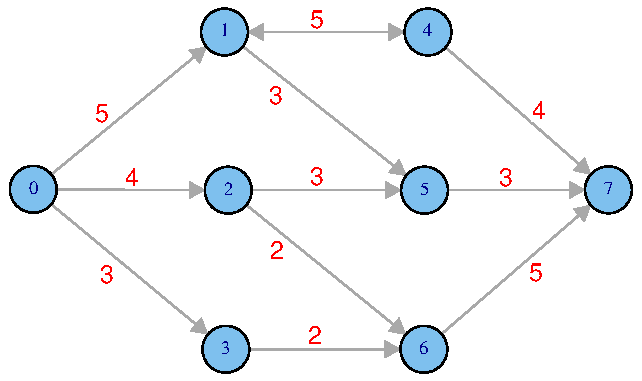
\includegraphics[width=8cm]{./pic/graph}
\caption{网络图}\label{fig:graph}
\end{figure}

\noindent{{\textbf  解:}这三个问题是图论中的典型问题。首先,应该在 \R 中构造该图,然后分别调用相关命令即可。
\R 代码及运行结果如下:}
\begin{Verbatim}
> library(igraph)                               #载入包
> e = matrix(nc = 3, byrow = TRUE, c(0,1,5, 0,2,4, 0,3,3, 1,5,3, 1,4,5,
+         2,5,3, 2,6,2, 3,6,2, 4,1,5, 4,7,4, 5,7,3, 6,7,5)) #边的权矩阵
> g = add.edges(graph.empty(8), t(e[,1:2]), weight = e[,3]) #构造图
> tkplot(g)                                     #绘制网络图
[1] 35
> graph.maxflow(g, 0,7, capacity = E(g)$weight) #最大流
[1] 11
> mst = minimum.spanning.tree(g)                #最小生成树
> tkplot(mst)                                   #绘制最小生成树
[1] 36
> (tree_min = sum(E(mst)$weight))               #计算并输出最小生成树的权
[1] 20
> shortest.paths(g, mode = "out")               #最短路矩阵
     [,1] [,2] [,3] [,4] [,5] [,6] [,7] [,8]
[1,]    0    5    4    3   10    7    5   10
[2,]  Inf    0  Inf  Inf    5    3  Inf    6
[3,]  Inf  Inf    0  Inf  Inf    3    2    6
[4,]  Inf  Inf  Inf    0  Inf  Inf    2    7
[5,]  Inf    5  Inf  Inf    0    8  Inf    4
[6,]  Inf  Inf  Inf  Inf  Inf    0  Inf    3
[7,]  Inf  Inf  Inf  Inf  Inf  Inf    0    5
[8,]  Inf  Inf  Inf  Inf  Inf  Inf  Inf    0
\end{Verbatim}
\begin{figure}[h]
\centering
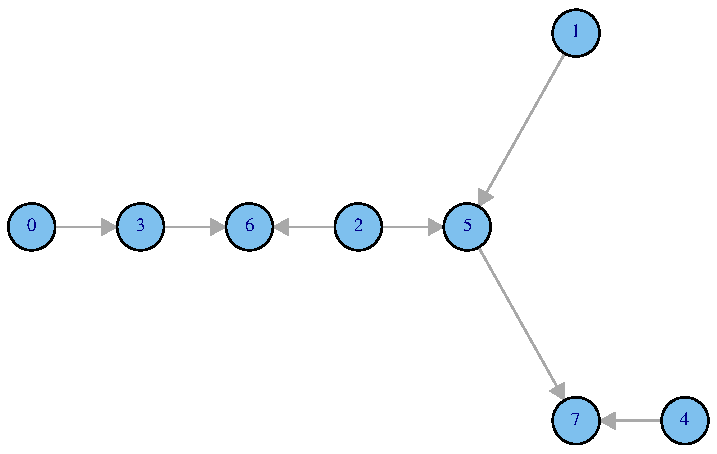
\includegraphics[width=8cm]{./pic/tree.pdf}
\caption{最小生成树图}\label{fig:tree}
\end{figure}

图 \ref{fig:graph} 为所画的网络图 (边上的数字由其它软件所绘)。图 \ref{fig:tree} 为最小生成树图。


由第 8 行可知,最大流为 11。由第 13 行可知,最小生成树的权为 20。由 15 -- 23 行 (最短路矩阵) 可以知道该网络上每
两个定点的最短路。如顶点 0 到顶点 7 的最短路为 10(矩阵中第 1 行第 8 列对应的元素)。需要说明的是,第 6,11 行结果
表示这是 \R 软件打开的第 35,36 个 tk 图形设备,与本题的具体内容无关。


观察以上代码和输出结果,发现 \R 仅仅用短短十行代码,就解决了最大流问题、最短路问题、最小生成树问题,并绘制出两个相关的
图形,其效率之高,令人叹为观止。而 LINGO 则需要针对每个问题输入不同模型、约束条件等,远远不如 \R 效率高,
至于绘图功能,LINGO 还需要很大的改进。
\subsection{专题:旅行商问题}
 旅行商问题即 TSP 问题 (travelling salesman problem):假设有一个人要游览 n 个城市,并且每个城市只能去一次,
 而且最后要回到原点,问他应该选取什么路线才能是总路线最短。旅行商问题易于描述但难于解决,是著名的 NP 难题之一 (有
  n 个城市时,路线组合数为 $(n-1)!/2$,组合数呈爆炸式增长),
 至今世界上还有不少人在研究它。解决该问题的算法也层出不穷,如动态规划、模拟退火算法、遗传算法、禁忌算法、蚁群算法等等。
 
 
 TSP 问题可分为对称型和非对称型两种,对称型即两地之间的距离没有方向性,即 a 地到 b 地的距离恒
 等于 b 地到 a 地的距离,而非对称问题中,则没有这个限制。\R 中,有专门解决 TSP 问题的包 \pkg{TSP} \citep{TSP08}。
 常用函数有 \fun{TSP()},\fun{ATSP()},\fun{solve\_TSP()},\fun{tour\_length()} 等。
 其中 \fun{TSP()} 和 \fun{ATSP()} 函数分别将对称矩阵、一般矩阵
处理为函数 \fun{solve\_TSP()} 所需要的数据格式。
\fun{solve\_TSP()} 为核心的求解函数,其用法为:

\begin{verbatim}
solve_TSP(x, method, control)
\end{verbatim}

其中,前两个参数比较常用,\rcode{x} 为 TSP 或 ATSP 格式,\rcode{method} 为所用的算法,选项有
 \rcode{nearest\_insertion}, \rcode{farthest\_insertion},
\rcode{arbitrary\_insertion},  \rcode{2-opt}, \rcode{nn} 等近十种
启发式算法\footnote{算法原理参见帮助文档。}。
%\rcode{arbitrary\_insertion}、\rcode{nn}、\rcode{repetitive\_nn}、
函数 \fun{tour\_length()} 计算所得路线的总长度。


由于 TSP 问题非常复杂,建议在解决规模较大 TSP 问题的的时候,不妨利用多种算法多次计算得到众多
 解后,再从中选择一个最好的作为最终解。下面结合具体例子来说明该函数的用法。
 \begin{exmp}\label{ex:path_china}
 走遍中国问题:你我周游全国,从北京出发,要遍游我国 34 个省级行政中心,最后要回到北京。假设各城市之间的
 路程可以视为它们在地球球面\footnote{地球为椭圆,但很近似于正圆,在这里将地球视为球体并不影响结果。}上的最短距离,
 请设计一条路线使得总行程最短。
 \end{exmp}

\noindent{{\textbf  解:}这是一个典型的对称 TSP 问题,通过组合数学知识,可知路线组合总数共有 $4.341659*10^{36}$ 种!}


 首先,获得 34 个省级行政中心的经纬度数据,
 根据空间几何知识,计算出它们两两之间的球面距离,然后调用 \pkg{TSP} 包中的相关函数即可得到最短路线。
 最后,还可以利用 \R 中的 \pkg{maps}\citep{maps08}, \pkg{maptools}\citep{maptools08}等包将所得路线以及城市画在中国地图上,
 得到一个直观、漂亮的结果。\R 代码如下:
 \VerbatimInput{./code/tsp.r}
 \begin{figure}[h]
\centering
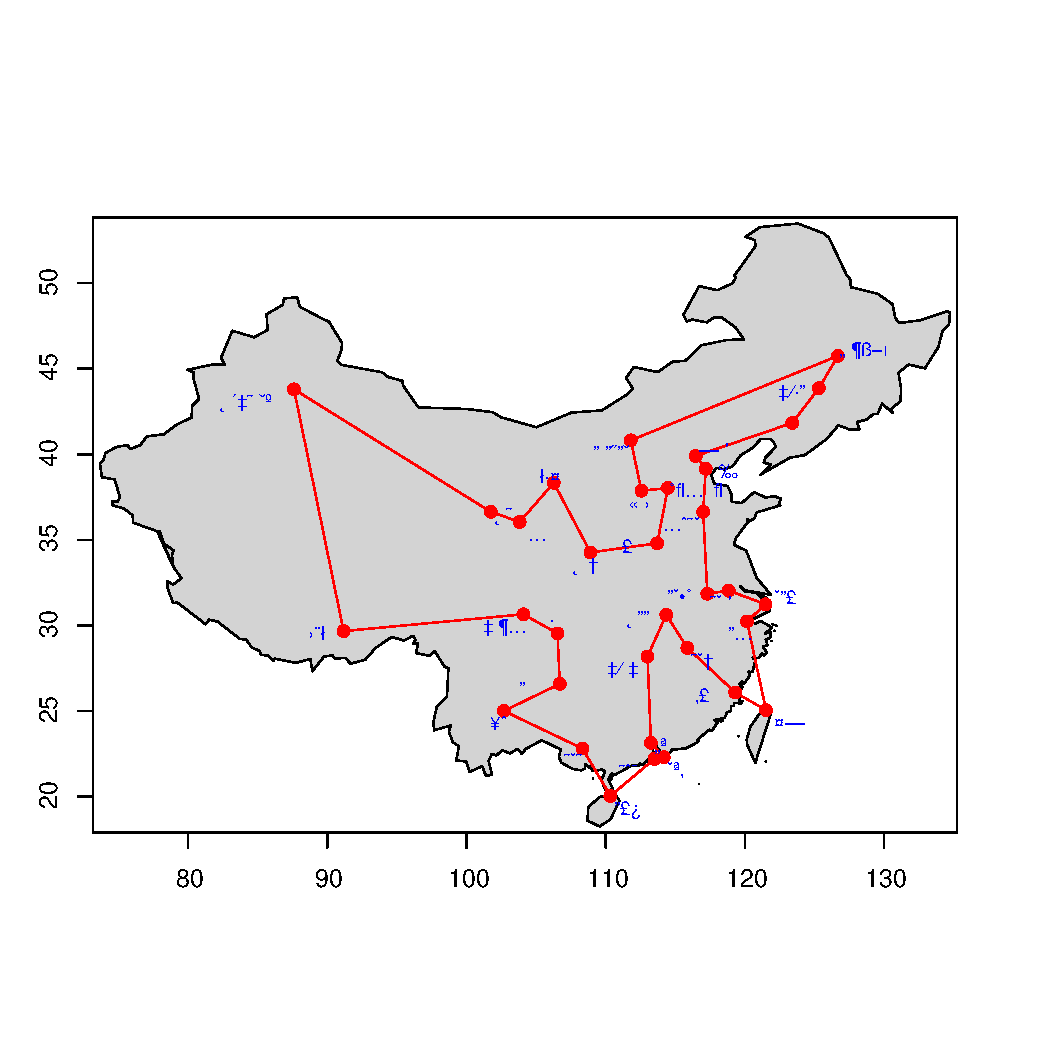
\includegraphics[width=12cm]{./pic/china.pdf}
\caption{走遍中国线路}\label{fig:path_china}
\end{figure}

上面程序中:第 4 行读取的 csv 格式
数据共有 3 列,分别为城市名、经度、纬度。
第 30 行中,\fun{pointLabel()} 函数将城市名标在地图上,
为了使它们重叠最小,该函数可以使用模拟退火算法 (默认) 或遗传算法来优化文本标签的放置位置。


多次运行程序,所得的最短路程\footnote{不能保证是全局最优解。}为 15638.01 千米,路线为
北京    、 天津    、 济南 、合肥    、 南京    、 上海 、杭州    、 台北    、 福州 、
南昌    、 武汉    、 长沙 、广州    、 香港    、 澳门 、海口    、 南宁    、 昆明 、
贵阳    、 重庆    、 成都 、拉萨    、 乌鲁木齐、 西宁 、兰州    、 银川    、 西安 、
郑州    、 石家庄  、 太原 、呼和浩特、 哈尔滨  、 长春 、沈阳    、 北京。
将路线画在中国地图上,如图 \ref{fig:path_china}。


另外,该包还提供了到 Concorde TSP Solver\footnote{需要单独下载,地址为 \url{http://www.tsp.gatech.edu/concorde/index.html}} 的接口,
Concorde TSP Solver 是一个专门解决 TSP 问题的开源软件包,有成功解决 15112 个城市的 TSP 问题的辉煌
战绩\footnote{根据斯特林公式,此时总的路线数约有 $15111!/2\approx4*10^{56593}$ 种。}。


通过此例,可以发现 \R 在读取数据、编程计算、绘图上都非常灵活强大 (熟悉 LINGO 软件的朋友应该更深有体会),
并且由于世界上各个领域内专家的无私贡献,\R 有了各种各样的包,可以便捷地解决各类问题。\R 不仅仅是一个统计软件,
而是一个由奉献者构建起来的平台,在这个平台上,我们可以随心所欲地解决各类问题,也可以将自己的优秀思想加进去。
众人拾柴火焰高,\R 的强大来自于大家。
%%%图与网络分析
 \section{结语}
 通过以上篇幅的讨论,可以初步领略 \R 在处理最优化问题时的强大之处,
 其语言之灵活、绘图之方便、涉及问题之全面,远胜于专门处理优化问题的 LINDO/LINGO 软件。
 工欲善其事,必先利其器,在最优化问题上,\R 绝对是一把倚天宝剑,而更令人惊讶而又惊喜的是,
 这把宝剑竟然是免费的!既然 \R 如此的价廉物美,那么在知识产权倍受重视的今天,
 我们又何必舍其粱肉,窃其糠糟呢?
 
 
 \R 中关于最优化的内容很多,本文涉及的仅是九牛一毛而已。作者殷切希望本文能够抛砖引玉,促进 \R 和最优化在国内的发展。

\section*{致谢}
首先感谢 \R 软件及各类包的所有作者,正因为他 (她) 们的无私奉献,才使得我们拥有 \R 这个卓越的软件。其次,我要感谢COS 论坛,是她让我认识了 \R 并提供了学习 \R 的便利。在本文的写作中,中国人民大学的谢益辉博士和南京大学的刘重杰老师
给了我莫大的鼓励和帮助,在此向他们致以崇高的敬意和由衷的感谢。
最后,我还要感谢我们寝室的所有兄弟,他们在生活上、学习上都给了我很大的帮助。


\begin{thebibliography}{20}
\newcommand{\enquote}[1]{``#1''}
\expandafter\ifx\csname natexlab\endcsname\relax\def\natexlab#1{#1}\fi
\expandafter\ifx\csname url\endcsname\relax
  \def\url#1{\texttt{#1}}\fi
\expandafter\ifx\csname urlprefix\endcsname\relax\def\urlprefix{URL }\fi
\providecommand{\eprint}[2][]{\url{#2}}

\bibitem[{胡运权(2007)}]{Op07}
胡运权 (2007).
\newblock \emph{运筹学教程}.
\newblock 清华大学出版社, 第三版 edition.
\newblock ISBN 978-7-302-14738-1.

\bibitem[{Berkelaar \emph{et~al.}(2008)}]{lpSolve08}
Berkelaar M, \emph{et~al.} (2008).
\newblock \emph{lpSolve: Interface to Lp\_solve v.5.5 to solve linear/integer
  programs}.
\newblock R package version 5.6.4.

\bibitem[{Csardi and Nepusz(2006)}]{igraph06}
Csardi G, Nepusz T (2006).
\newblock \enquote{The igraph software package for complex network research.}
\newblock \emph{InterJournal}, \textbf{Complex Systems}, 1695.
\newblock \urlprefix\url{http://igraph.sf.net}.

\bibitem[{Hahsler and Hornik(2008)}]{TSP08}
Hahsler M, Hornik K (2008).
\newblock \emph{TSP: Traveling Salesperson Problem (TSP)}.
\newblock R package version 0.2-4,
  \urlprefix\url{http://r-forge.r-project.org/projects/tsp/}.

\bibitem[{Lewin-Koh \emph{et~al.}(2008)Lewin-Koh, Bivand, contributions~by
  Edzer J.~Pebesma, Archer, Dray, Forrest, Giraudoux, Golicher, Rubio,
  Hausmann, Jagger, Luque, MacQueen, Niccolai, and Short}]{maptools08}
Lewin-Koh NJ, Bivand R, contributions~by Edzer J~Pebesma, Archer E, Dray S,
  Forrest D, Giraudoux P, Golicher D, Rubio VG, Hausmann P, Jagger T, Luque SP,
  MacQueen D, Niccolai A, Short T (2008).
\newblock \emph{maptools: Tools for reading and handling spatial objects}.
\newblock R package version 0.7-15.

\bibitem[{Minka(2008)}]{maps08}
Minka TP (2008).
\newblock \emph{maps: Draw Geographical Maps}.
\newblock R package version 2.0-40.

\bibitem[{Novomestky(2008)}]{goalprog08}
Novomestky F (2008).
\newblock \emph{goalprog: Weighted and lexicographical goal programming and
  optimization}.
\newblock R package version 1.0-2.

\bibitem[{{R Development Core Team}(2008)}]{R08}
{R Development Core Team} (2008).
\newblock \emph{R: A Language and Environment for Statistical Computing}.
\newblock R Foundation for Statistical Computing, Vienna, Austria.
\newblock {ISBN} 3-900051-07-0, \urlprefix\url{http://www.R-project.org}.

\bibitem[{Tamura(2007)}]{Rdonlp207}
Tamura R (2007).
\newblock \emph{Rdonlp2: an R extension library to use Peter Spelluci's DONLP2
  from R.}
\newblock R package version 0.3-1, \urlprefix\url{http://arumat.net/Rdonlp2/}.

\bibitem[{Tendys(2002)}]{gafit02}
Tendys T (2002).
\newblock \emph{gafit: Genetic Algorithm for Curve Fitting}.
\newblock R package version 0.4,
  \urlprefix\url{http://www.progsoc.uts.edu.au/~telford/}.

\bibitem[{Theussl and Hornik(2008)}]{Rglpk08}
Theussl S, Hornik K (2008).
\newblock \emph{Rglpk: R/GNU Linear Programming Kit Interface}.
\newblock R package version 0.2-5,
  \urlprefix\url{http://R-Forge.R-project.org/projects/rglp/,
  http://www.gnu.org/software/glpk/}.

\bibitem[{Winston(2007)}]{OP06}
Winston WL (2007).
\newblock \emph{运筹学--应用范例与解法}.
\newblock 清华大学出版社, 第四版 edition.
\newblock ISBN 7-302-13208-9/TP·8347.

\end{thebibliography}


\end{document}
